% Created 2021-01-13 Wed 15:53
% Intended LaTeX compiler: pdflatex
\documentclass[11pt]{article}
\usepackage[utf8]{inputenc}
\usepackage[T1]{fontenc}
\usepackage{graphicx}
\usepackage{grffile}
\usepackage{longtable}
\usepackage{wrapfig}
\usepackage{rotating}
\usepackage[normalem]{ulem}
\usepackage{amsmath}
\usepackage{textcomp}
\usepackage{amssymb}
\usepackage{capt-of}
\usepackage{hyperref}
\usepackage{minted}
\usepackage[a4paper,margin=20mm]{geometry}
\usepackage{amsmath}
\usepackage{amsfonts}
\usepackage{bm}
\usepackage{minted}
\usemintedstyle{emacs}
\usepackage[T1]{fontenc}
\usepackage[scaled]{beraserif}
\usepackage[scaled]{berasans}
\usepackage[scaled]{beramono}
\newcommand{\tr}{\textsf{T}}
\newcommand{\grad}{\bm{\nabla}}
\newcommand{\av}[2][]{\mathbb{E}_{#1\!}\left[ #2 \right]}
\newcommand{\Prob}[2][]{\mathbb{P}_{#1\!}\left[ #2 \right]}
\newcommand{\logg}[1]{\log\!\left( #1 \right)}
\newcommand{\e}[1]{{\rm e}^{#1}}
\newcommand{\dd}{\mathrm{d}}
\DeclareMathAlphabet{\mat}{OT1}{cmss}{bx}{n}
\newcommand{\normal}[2]{\mathcal{N}\!\left(#1 \big| #2 \right)}
\newcounter{eqCounter}
\setcounter{eqCounter}{0}
\newcommand{\explanation}{\setcounter{eqCounter}{0}\renewcommand{\labelenumi}{(\arabic{enumi})}}
\newcommand{\eq}[1][=]{\stepcounter{eqCounter}\stackrel{\text{\tiny(\arabic{eqCounter})}}{#1}}
\newcommand{\argmax}{\mathop{\mathrm{argmax}}}
\author{Adam Prügel-Bennett}
\date{\today}
\title{Designing a Network}
\hypersetup{
 pdfauthor={Adam Prügel-Bennett},
 pdftitle={Designing a Network},
 pdfkeywords={},
 pdfsubject={},
 pdfcreator={Emacs 26.3 (Org mode 9.1.9)}, 
 pdflang={English}}
\begin{document}

\maketitle

\section{Overall Design}
\label{sec:org28952ba}
\begin{center}
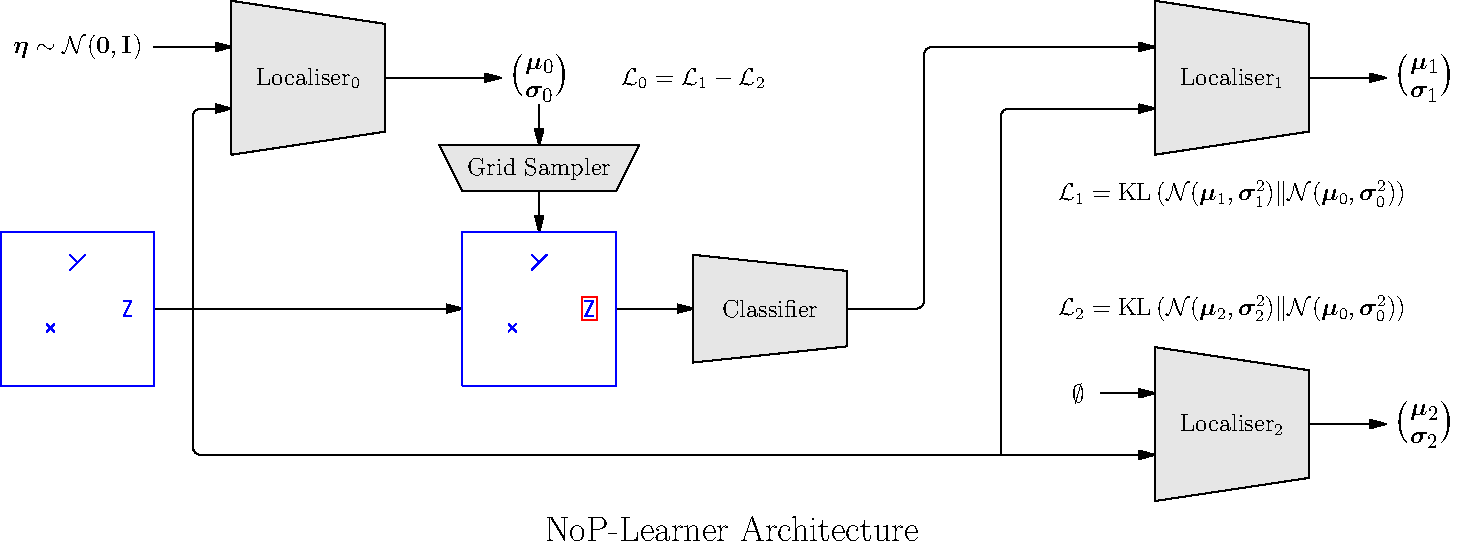
\includegraphics[width=.9\linewidth]{./figures/nopArchitecture.pdf}
\end{center}

\begin{itemize}
\item Localisers differ by attention unit
\item Use of \texttt{affine\_grid} and \texttt{grid\_sampler} to sample a local part of
image
\item Converting \((x,y,\sigma_x,\sigma_y)\) to affine parameters
\(\begin{pmatrix} \sigma_x & 0 & x\\ 0 & \sigma_y& y\end{pmatrix}\)
\end{itemize}
\begin{minted}[]{python}
import torch
import torch.nn.functional as F
b = 3;                 # batch size
h = w = 4;
c = 3;
images = torch.rand([b,c,h,w])
newHeight = newWidth

t = torch.rand([b,4])  # example output for localiser0
toAffine = torch.tensor([[[0.0,0,1,0],[0,0,0,0],[1,0,0,0]],[[0,0,0,0],[0,0,0,1],[0,1,0,0]]])
a=torch.einsum("xyz,bz->bxy", [toAffine,t])
grid = F.affine_grid(a, [b,c,newHeight,newWidth])
newImages = F.grid_sample(images, grid)
\end{minted}

\section{Localiser}
\label{sec:org72fc6f0}
\begin{center}
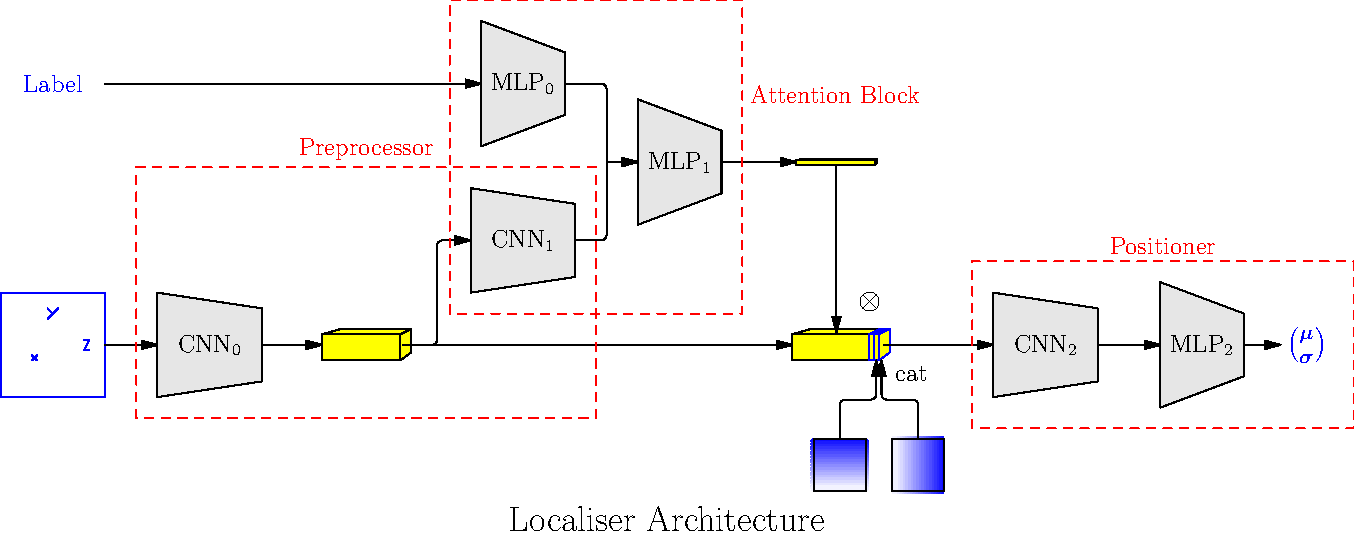
\includegraphics[width=.9\linewidth]{./figures/localiser.pdf}
\end{center}

\begin{itemize}
\item CNN\(_{\text{0}}\), CNN\(_{\text{1}}\), CNN\(_{\text{2}}\) and MLP\(_{\text{3}}\) are all shared between localisers
\item They differ only in the attention block and there only in MLP\(_{\text{1}}\)
and MLP\(_{\text{2}}\)
\item Number of channels output by CNN\(_{\text{0}}\) will depend on complexity of input
\begin{itemize}
\item (c, w, h) = (16,16,16) seems reasonable
\end{itemize}
\end{itemize}

\subsection{Preprocessor}
\label{sec:org77cb49e}
\_ This is CNN\(_{\text{0}}\) and CNN\(_{\text{1}}\)
\begin{itemize}
\item Turns input image into 16x16x16 tensor
\item This is split into two parts
\end{itemize}
\subsubsection{Preprocessor part 1}
\label{sec:orgdf68b3b}
\begin{itemize}
\item CNN1

\begin{center}
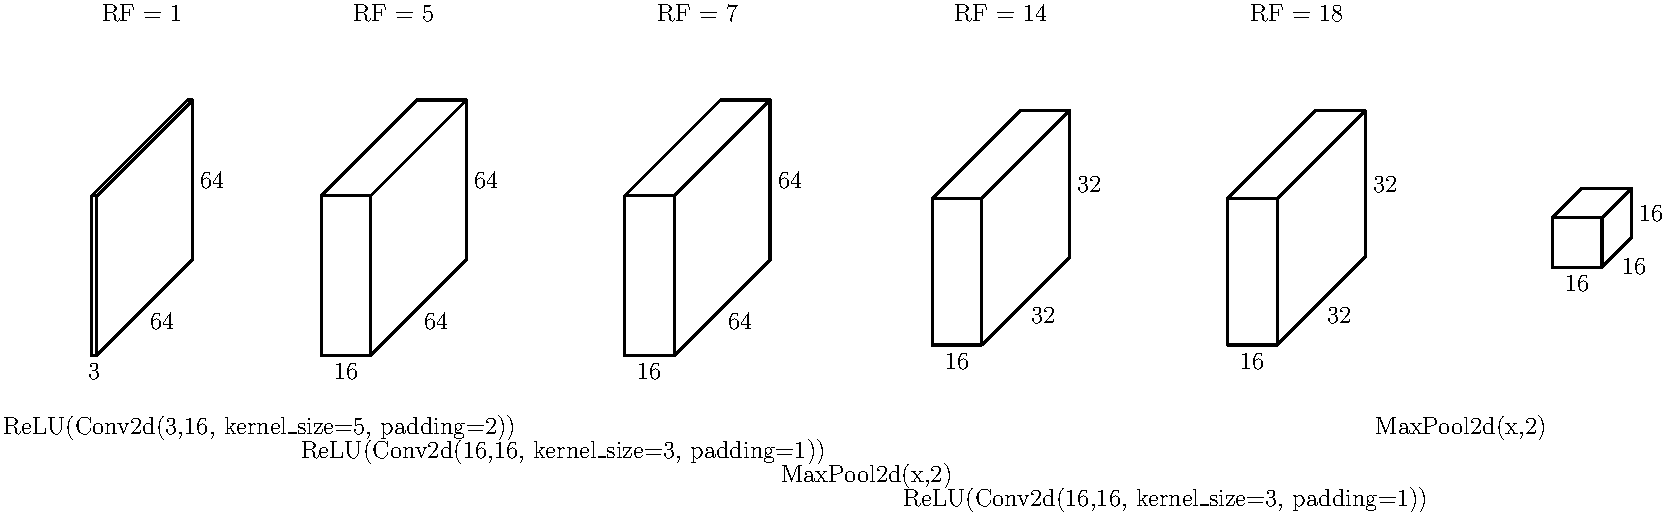
\includegraphics[width=.9\linewidth]{./figures/preprocessor.pdf}
\end{center}
\end{itemize}
\begin{minted}[]{python}
# init
	def __init__(self):
		super(Net, self).__init__()
		self.conv1 = nn.Conv2d(3,16, kernel_size=5, padding=2)
		self.conv2 = nn.Conv2d(16,16, kernel_size=3, padding=1)
		self.conv3 = nn.Conv2d(16,16, kernel_size=3, padding=1)

# forward
	def forward(self, x):
		x = F.relu(self.conv1(x))
		x = F.max_pool2d(F.relu(self.conv2(x)), 2)
		x = F.max_pool2d(F.relu(self.conv3(x)), 2)
		return x
\end{minted}

\subsubsection{Preprocessor Part 2}
\label{sec:org8928489}
\begin{itemize}
\item This is CNN\(_{\text{1}}\)
\begin{center}
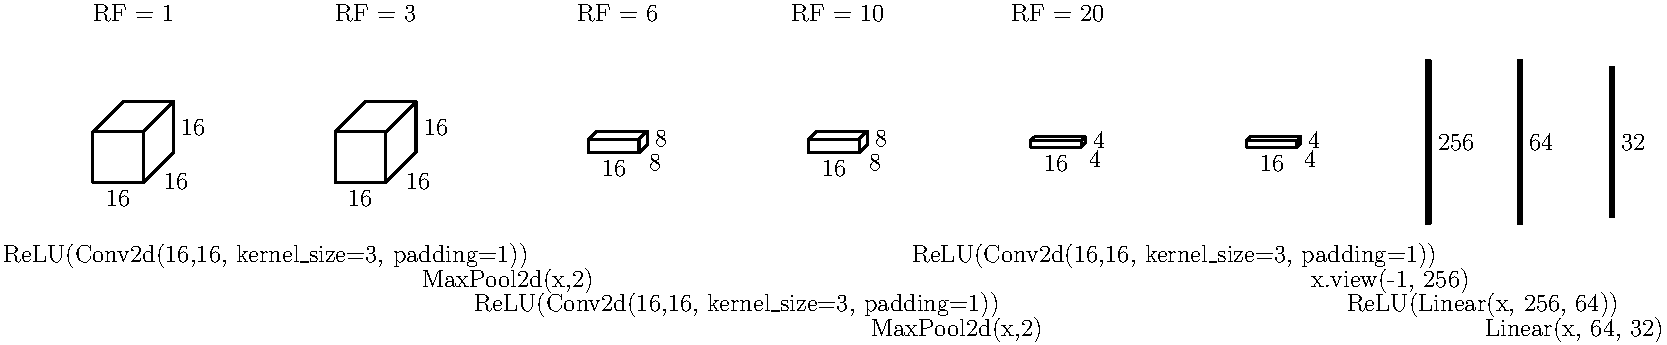
\includegraphics[width=.9\linewidth]{./figures/preprocessor2.pdf}
\end{center}
\end{itemize}
\begin{minted}[]{python}
# init
	def __init__(self):
		super(Net, self).__init__()
		self.conv1 = nn.Conv2d(16,16, kernel_size=3, padding=1)
		self.conv2 = nn.Conv2d(16,16, kernel_size=3, padding=1)
		self.conv3 = nn.Conv2d(16,16, kernel_size=3, padding=1)
		self.fc1 = nn.linear(256, 64),
		self.fc2 = nn.linear(64, 32),

# forward
	def forward(self, x):
		x = F.max_pool2d(F.relu(self.conv1(x)), 2)
		x = F.max_pool2d(F.relu(self.conv2(x)), 2)
		x = F.relu(self.conv3(x))
		x = x.view(-1, 256)
		x = F.relu(self.fc1(x))
		x = self.fc2(x)
		return x

\end{minted}

\subsection{Positioner}
\label{sec:orge13452d}
\begin{itemize}
\item This is CNN\(_{\text{2}}\) and MLP\(_{\text{3}}\)
\item Takes output from preprocessor and attention and returns 
pos=[\(\mu_{\text{x,}\mu}\)\(_{\text{y,}\sigma}\)\(_{\text{x,}\simga}\)\(_{\text{y}}\)]
\end{itemize}
\begin{itemize}
\item Concatenate two feature maps with x and y position using
torch.cat (see  \href{https://eng.uber.com/coordconv/}{CoordConv}])
\end{itemize}

\begin{minted}[]{python}
import torch
w = 4 # assuming h=w
b = 2
c = 3
ones = torch.ones(w)
seq = torch.linspace(0,1,w)
colCoord = torch.einsum("a,b->ab", [ones,seq]).repeat(b,1,1,1)
rowCoord = torch.einsum("a,b->ab", [seq,ones]).repeat(b,1,1,1)
t = torch.ones([b,c,w,w])
tcat = torch.cat((t,colCoord,rowCoord), dim=1)
print(tcat)
\end{minted}

\begin{itemize}
\item CNN2, MLP2
\begin{center}
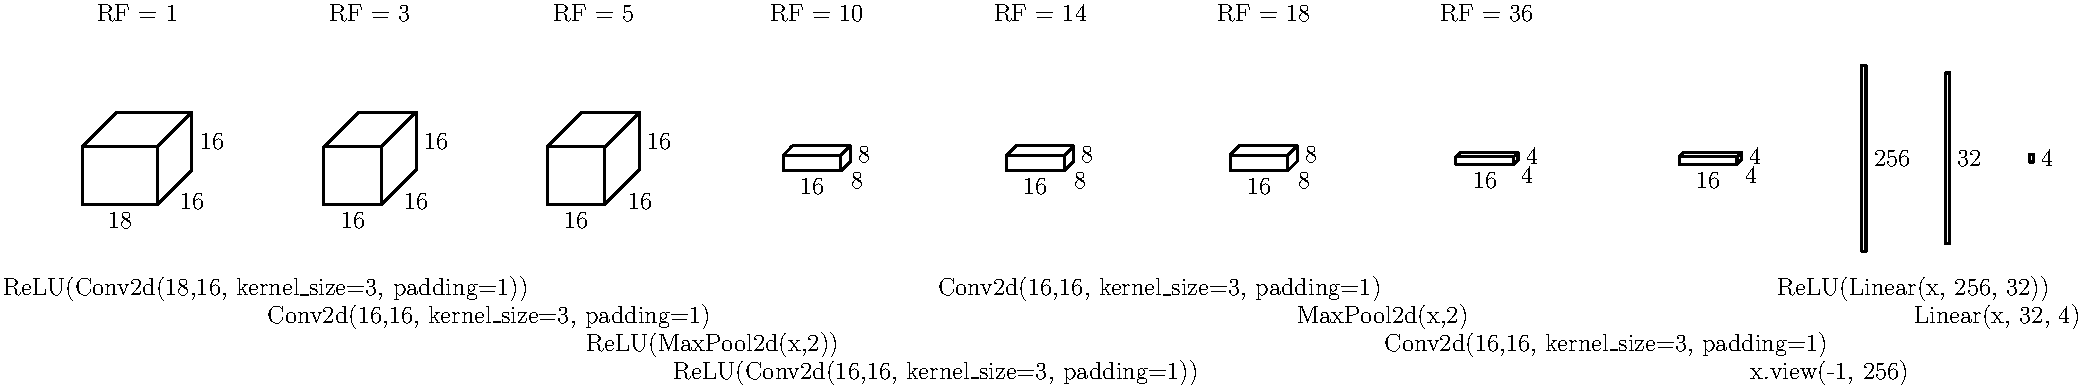
\includegraphics[width=.9\linewidth]{./figures/positioner.pdf}
\end{center}
\end{itemize}

\begin{minted}[]{python}
# init
	def __init__(self):
		super(Net, self).__init__()
		self.conv1 = nn.Conv2d(18,16, kernel_size=3, padding=1)
		self.conv2 = nn.Conv2d(16,16, kernel_size=3, padding=1)
		self.conv3 = nn.Conv2d(16,16, kernel_size=3, padding=1)
		self.conv4 = nn.Conv2d(16,16, kernel_size=3, padding=1)
		self.conv5 = nn.Conv2d(16,16, kernel_size=3, padding=1)
		self.fc1 = nn.linear(256, 32),
		self.fc2 = nn.linear(32, 4),

# forward
	def forward(self, x):
		x = F.relu(self.conv1(x))
		x = F.relu(F.max_pool2d(self.conv2(x), 2))
		x = F.relu(self.conv3(x))
		x = F.max_pool2d(self.conv4(x), 2)
		x = self.conv5(x)
		x = x.view(-1, 256)
		x = F.relu(self.fc1(x))
		x = self.fc2(x)
		return x

\end{minted}

\subsection{Attention Module}
\label{sec:orgf4b668d}
\begin{itemize}
\item With no input (Locaiser\(_{\text{2}}\)) we don't have MLP\(_{\text{1}}\)
\item Number of outputs = Number of feature sets (channels)
\item Multiply channels by output
\end{itemize}
\begin{minted}[]{python}
import torch
t = torch.ones([2,3,4,4])
print(t)
att = torch.tensor([[1,2,3],[2,3,4]])
ta = torch.einsum("bcwh,bc->bcwh", [t,att])
print(ta)
\end{minted}

\section{Loss functions}
\label{sec:org9ed8367}
We consider three sets of parameters
\begin{enumerate}
\item Localisation parameters, Classifier and Attention1
\begin{itemize}
\item Minimise \(\mathcal{L}_1 = \mathrm{KL}(q_0\|q_1)\)
\end{itemize}
\item Attention2
\begin{itemize}
\item Minimise \(\mathcal{L}_2 = \mathrm{KL}(q_0\|q_2)\)
\end{itemize}
\item Attention0
\begin{itemize}
\item Minimise \(\mathcal{L}_1 - \mathcal{L}_2\)
\end{itemize}
\end{enumerate}

\subsection{KL-losses}
\label{sec:org877e2ff}
\begin{itemize}
\item KL-divergence  for general probabilities

\[ \mathrm{KL}(q_0\|q_1) = \int q_0(\bm{x}) \,
     \logg{\frac{q_0(\bm{x})}{q_1(\bm{x})}} \, \dd x \]

\item Two normals

\[\mathrm{KL}(q_0\|q_1) = \frac{1}{2} \left(
     \frac{\sigma_0^2}{\sigma_1^2} - 1 -
     \logg{\frac{\sigma_0^2}{\sigma_1^2}} +
     \frac{(\mu_0-\mu_1)^2}{\sigma_1^2} \right) \]

\item I prefer to output \(\sigma_i\) as it is dimensionally meaningful.
Also I know that \(0<\sigma_i<1\) so I can put this through a sigmoid
\end{itemize}




\begin{minted}[]{python}
kl_loss = 0.5 * torch.sum(torch.exp(z_var) + z_mu**2 - 1. - z_var)
\end{minted}



\section{Classifier}
\label{sec:orgf39c126}
\begin{itemize}
\item Input: 16x16 subimage
\item The classifier is a small CNN using Gumbel softmax
\href{https://pytorch.org/docs/stable/\_modules/torch/nn/functional.html\#gumbel\_softmax}{pytorch code}
\href{https://pytorch.org/docs/stable/nn.functional.html\#gumbel\_sofmax}{pytorch docs}
\item We can experiment with multiple outputs as an example of disentanglement
\item Assuming sub-images of size (3,16,16)
\begin{center}
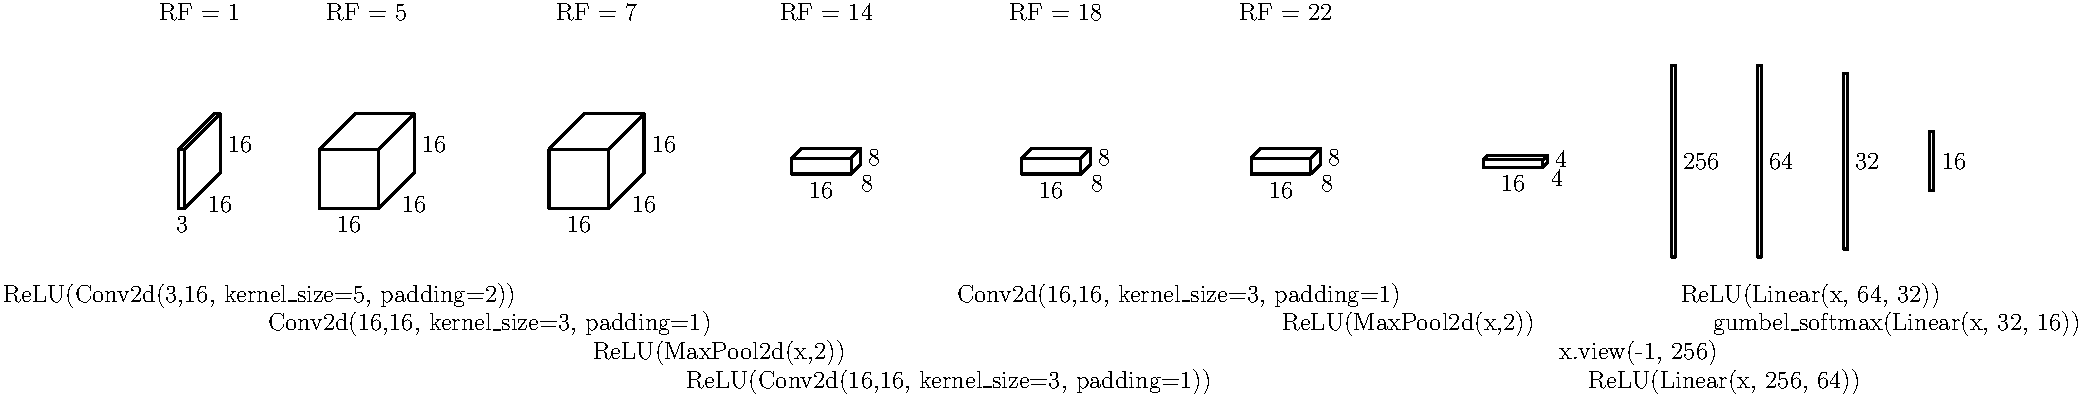
\includegraphics[width=.9\linewidth]{./figures/classifier.pdf}
\end{center}
\end{itemize}

\begin{minted}[]{python}
import torch
import torch.nn as nn
import torch.nn.functional as F

NoInChannels = 3;

class Classifier(nn.Module):

	def __init__(self):
		super(Classifier, self).__init__()
		self.conv1 = nn.Conv2d(NoInchannels,16, kernel_size=5, padding=2)
		self.conv2 = nn.Conv2d(16,16, kernel_size=3, padding=1)
		self.conv3 = nn.Conv2d(16,16, kernel_size=3, padding=1)
		self.conv4 = nn.Conv2d(16,16, kernel_size=3, padding=1)
		self.fc1 = nn.Linear(256, 64)
		self.fc2 = nn.Linear(64, 32)
		self.fc3 = nn.Linear(32, 16)

	def forward(self, x):
		x = F.relu(self.conv1(x))
		x = F.relu(F.max_pool2d(self.conv2(x), 2))
		x = F.relu(self.conv3(x))
		x = F.relu(F.max_pool2d(self.conv4(x), 2))
		x = x.view(-1, 256)
		x = F.relu(self.fc1(x))
		x = F.relu(self.fc2(x))
		x = F.gumbel_softmax(self.fc3(x), hard=True)
		return x

classifier = Classifier();

batchsize = 3

x = torch.rand([batchsize, NoInChannels, 16, 16)

to = classifier.forward(x)
to.shape
\end{minted}


\section{Datasets}
\label{sec:org663c67b}
\begin{itemize}
\item MultiMNist
\begin{itemize}
\item 256x256
\end{itemize}
\item CLEVR
\begin{itemize}
\item 128x128
\end{itemize}
\item Coco
\end{itemize}
\end{document}
